\documentclass[conference]{IEEEtran}
\usepackage{fancyhdr}\usepackage[utf8]{inputenc}
\usepackage{graphicx}
\usepackage{multirow}

\usepackage{lastpage}

%\usepackage{draftwatermark}


%\SetWatermarkText{UoA}
%\SetWatermarkScale{3}

\pagestyle{fancy}
\fancyhf{}
\rfoot{Page \thepage \hspace{1pt} of \pageref{LastPage}} 

\title{Is it Possible to Extend IPv6?}
\date{December 2022}

\author{\IEEEauthorblockN{Ana Custura}
\IEEEauthorblockA{
\textit{University of Aberdeen}\\
}
\and
\IEEEauthorblockN{Raffaello Secchi}
\textit{University of Aberdeen}\\
\and
\IEEEauthorblockN{Gorry Fairhurst}
\textit{University of Aberdeen}\\
}
\begin{document}

\maketitle

\begin{abstract}
The IPv6 Hop-by-Hop Options and Destination Options Extension Headers have historically faced challenges in deployment due to the lack of support in hardware-based forwarding and concerns around potential denial-of-service attacks. However, there has been a renewed interest within the standards community both in simplifying their processing, and in using them for new applications. 
Through a wide-scale measurement campaign, we show that many autonomous systems in access networks and core of the Internet permit the traversal of EHs including Options, and that path traversal depends on the type of network, size of Option and transport protocol used, but does not depend on the type of Option included. We show that packets including Extension Headers can impact load balancing network functions, and present evidence of equipment mis-configuration. Finally, we outline the current deployment challenges  and provide recommendations for utilizing new Options to extend IPv6.

\end{abstract}

\begin{IEEEkeywords}
IPv6 protocol, Extension Headers, Protocol Evolution, Destination Options, Hop-by-hop Options
\end{IEEEkeywords}

\section{Introduction}
\label{sec:introduction}

IPv6 Extension Headers (EHs)~\cite{RFC8200} are optional headers that a source node can
add to the base IPv6 header to include extra functionality and features as a packet traverses an IPv6 network path. They were defined in the IPv6 specification
to ensure the protocol was flexible and extensible.
%The use of extension headers allows for a flexible and extensible design of IPv6 that can support a variety of new networking features and technologies.
% commented out as it does not say much
IPv6 EHs are widely used to implement specific functions. 
However, in this paper we focus on network support for two key EHs: the Destination Options (DST) header and the Hop-by-Hop Options (HBH) header~\cite{rfc9098}, as they are the primary means to extend IPv6 functions.


Recent presentations to the networking community have commented on the limited path traversal of packets including EHs and remarked that network devices, such as firewalls, routers, load balancers and intrusion detection systems~\cite{nalini-iepg114, fernando-talk} do not properly handle packets including an EH. This can result in a drop of the packet including the EH (i.e., the packet fails traverse the end-to-end network path).

Additionally, some network administrators may use firewalls to implement Access Control Lists (ACLs) at the outer edge of access and enterprise networks, which discard packets including an EH. This is done to mitigate security concerns, such as bypassing security mechanisms or defending against denial-of-service (DoS) attacks~\cite{naagas2021deh}.


Plausible reasons for limited traversal of packets including EHs are documented in~\cite{ietf-v6ops-hbh-03}, where the authors note that early IPv6 routers
processed EHs in software. This processing of EHs would normally utilise the slow-path, rather than the optimised fast-path, resulting in decreased router forwarding rates. In some designs, this processing consumed resources that would normally be used for Control Plane processing, opening up a potential DoS attack vector on the critical router functions (reducing ability to perform routing, management, etc). This motivated network operators to implement policies to drop packets that include EHs~\cite{rfc9098}.  This, in turn,
discouraged use of EHs and their successful standardisation. 

However, important recent changes motivate the need to take a fresh look at the usability of EHs as a mechanism to extend IPv6: modern high-speed routers have introduced flexible forwarding hardware that can support the ability to parse and process simple headers within the fast-path~\cite{programmable-data-plane, cisco-silicon-one, hauser2023}; and specific use-cases have emerged where there is an operational demand for new techniques that could be realised through EHs.

%XXX at some point here we will include a ref to ASIC XXX

The paper provides insight into whether these changes in operations and equipment have impacted the forwarding of packets that include the HBH and DST EHs, and seeks to understand the opportunity to use these EHs to implement new functions. It begins by discussing previous independent measurements that have reported variable results on the traversal of IPv6 packets that include an EH~\cite{RFC7872} \cite{apnic} \cite{nalini-iepg114} \cite{james}.
It then presents a broad dataset collected to explore key aspects (e.g., the size of the EH, the choice of transport, and choice and composition of the EH Options), revealing a more diverse and nuanced picture of Internet paths than was previously reported.

%XXX Unsure I think the next para is well placed, nor necesarily the correct story ... the shape of this depends on journal style XXX

Specifically, the results demonstrate that if  EHs are limited in size,
packets including a DST EH can traverse as many as
95\% of a diverse set of Internet paths. While HBH EH packets only traverse a narrow set of paths, when we
characterise whether packets traverse Autonomous Systems (AS), if we exclude operator policies in access and transit networks, we find many ASes forward packets that include this type of EH.

This paper also presents novel insights into the forwarding of packets that include a DST or HBH EH. Our research findings
demonstrate that the inclusion of some EHs in packets on paths with a form of network layer load-balancing often results in a narrower set of forwarding paths. Although one could interpret this as an alternative approach to extracting entropy from EHs, it is more likely a
pathological outcome of load balancing network routers not configured to support packets that include EHs.
We recpmmend that eliminating these pathologies would open up opportunities for
developers and network operators to take advantage of a range of recently-standardised or in-progress innovative ideas based on EHs, such as tools to monitor network performance~\cite{rfc8250}~\cite{ietf-ippm-ioam-ipv6-options-10} or enabling larger packets~\cite{rfc9268}.

%XXX Summary para below XXX

The remainder of this paper is organised as follows:  Section~\ref{sec:background} presents
the required background for IPv6 EHs and describes the historical challenges related to their deployment.  The previous literature describing measurement of paths using packets including IPv6
EHs is surveyed in Section~\ref{sec:motivation}.
Sections~\ref{sec:methodology}-\ref{sec:pathspider-results} present the
methodology and results of this study, organised by the type of network path.  The
implications of our results are discussed in Section~\ref{sec:discussion}.
Finally, the conclusion summarises our findings.

\section{Extending IPv6}
\label{sec:background}

%%XXX EH or OPT????????

\label{sec:ipv6-option-deployment}

\begin{figure}
\centering
  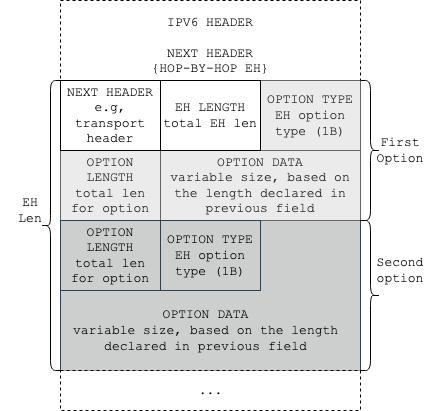
\includegraphics[width=0.5\textwidth]{ehformat.png}
  \caption{IPv6 packet with a base header that includes two EHs}
  \label{fig:eh-format}
\end{figure}


The original IPv6 specification~\cite{rfc2460} introduced a flexible header structure consisting of a fixed-length base header and one or more optional Extension Headers (EHs). 
IPv6 became a full standard in 2017~\cite{RFC8200}. This updated RFC 2460, and also changed some of the processing rules for EHs to align with the current operational practice. RFC 8200~\cite{RFC8200} allows multiple EHs in a single packet providing that they can fit the first fragment in case of fragmentation. 

The type of the first EH is denoted in the Next Header field of the IPv6 base header. Each consecutive EH contains a Next Header field to specify the type of the following EH, forming a chain terminated by the IPv6 payload. Each EH also contains a Length field specifying its total length. 

Besides HBH and DST, the types of EH include Routing, Fragment, and
Authentication and the Encapsulating Security Payload Header.
The Fragment header, Authentication and Encapsulating Security Payload header operate end-to-end and follow the Routing header if present. 

When a HBH EH is included, it must be placed immediately after the base header~\cite{RFC8200}.  The DST EH is the only EH which is permitted to be included more than once (i.e., it can appear before and after the Routing EH). 

The Routing EH is widely used by SRv6 to ensure the path includes specified intermediate nodes, typically within a single domain. SRv6 is currently deployed and actively researched~\cite{srv6}~\cite{srperf}.
Since the HBH (and first DST) come before the Routing EH, they have to be processed or skipped for routers that act as SRv6 intermediate nodes, to allow them to update the destination address using the Routing EH.

The final place a DST EH can appear is directly before the payload and is meant to be consumed at the final destination endpoint. This is propagated transparently over a network path. The DST and HBH EHs are the primary means by which IPv6 functions can be extended, by defining new Options.


Options use a Type-Length-Value (TLV) encoding~\cite{RFC8200} with 1~byte for each of the Type and Length fields, and a variable-sized Value field that carries the Option data. Their total length is always a multiple of 8 bytes to preserve alignment. Figure~\ref{fig:eh-format} shows the structure of an IPv6 packet including a base header followed by a HBH EH containing two Options.


A router can skip any Options that it does not understand. In addition, when an Option is unknown, the two most significant bits of the Type
specify the action a router should take to address the unrecognised header. When the two most significant bits are 00, the router should
ignore the Option and continue processing the header. If these bits are 01, the
processing should stop and discard the packet. If the bits are 10,
the packet should be discarded and an ICMP notification should be returned to
the sender. Finally, if the bits are 11, the same actions as for 10 should occur,
but this notification should be sent only if the destination address was not multicast. 

Table~\ref{tbl:options} presents the currently standardised 
Options.  We observe that most Options set the two most significant bits
(MSBs) to 00.  The third most significant bit specifies, if set, that the Option data field can be modified en route.

Because HBH Options can be modified by routers on a path, they can be used to provide and collect data from routers to support measurement. This has opened up opportunities for innovative alternatives to traditional mechanisms for measurement (e.g., using ICMP): Option 0x30 provides additional input to inform  PMTUD or PLPMTUD~\cite{rfc9268}, Option 0x12 has been specified to measure packet loss, latency, and jitter on live traffic measurement~\cite{rfc9343} and recently-proposed Option 0x31 records operational and telemetry information that can be updated by routers on then path between two endpoints.
Originally, all routers on a path were required to examine and process the HBH EH~\cite{rfc2460}. This requirement was realxed by~\cite{RFC8200} to only require processing when support is  configured.


DST can carry Options that provide similar functionality. Option 0x0F~\cite{rfc8250} can be used to measure performance and provide diagnostic metrics such as round-trip delay. 


% The total EH length is 8-byte aligned and specified in the
% EH Length field, while each individual option declares its own length in the
% Option Length field. 

\begin{table}[b]
\center
\caption{Currently Standardised DST and HBH Options.}
\begin{tabular}{p{0.03\textwidth}|p{0.055\textwidth}|l|p{0.18\textwidth}}
Hex  & MSBs & Type      & Description                                              \\
\hline
\hline
0x00 & 000  & HBH, Dest & Pad1 (padding)                                           \\
0x01 & 000  & HBH, Dest & PadN (padding)                                           \\
0xC2 & 110  & HBH       & Enable jumbo payloads                                    \\
0x23 & 001  & HBH       & Low-Power and Lossy Networks routing                     \\
0x04 & 000  & Dest      & Mechanism for IPv6 encapsulation                 \\
0x05 & 000  & HBH       & Mechanism for requesting router processing, Router Alert              \\
0xC9 & 110  & Dest      & Mobility Support in IPv6                                 \\
0x8C & 100  & Dest      & Method for identifying subscribers in broadband networks \\
0x6D & 011  & HBH       & Multicast Protocol for Low-Power and  Lossy Networks     \\
0x0F & 000  & Dest      & Delay measurement                                        \\
0x30 & 001  & HBH       & PathMTU                                     \\
0x11 & 000  & HBH, Dest & \multirow{2}{*}{On-path operational info}                \\
0x31 & 001  & HBH, Dest &                                                          \\
0x12 & 000  & HBH, Dest & On-path telemetry                                       
\end{tabular}
  \label{tbl:options}
\end{table}


\subsection{Previous Studies of IPv6 EHs}

\label{sec:motivation}

The debate on whether or not IPv6 packets that include EHs traverse the Internet is not new to the Internet community.
In 2015, an Informational IETF document presenting traceroute active
measurements to destinations within the Alexa top 1M domains~\cite{RFC7872}
revealed that packets including EHs experience a significantly higher drop rate over an
Internet path compared to packets that do not include EHs. Since then, other
studies~\cite{james}~\cite{nalini-iepg114}~\cite{apnic} have appeared within the standards community that support this claim.  However,
the level and nature of the reported loss varied significantly in these
reports.  This suggests the need for more analysis into the causes of loss and the need to define new measurement methods~\cite{james}~\cite{elkins-v6ops-eh-deepdive-fw-01}.  


Another IETF draft, ``Just Another Measurement of Extension header
Survivability" (JAMES)~\cite{james}, presents results for EH path traversal using
traceroute measurements over a mesh network with 21 vantage points located in a set of globally distributed Autonomous Systems (ASes). This study tests all the standard EHs
(including Routing, Fragment, etc.) in a setting where both ends of the
communication path are under the control of the researcher.  It reported traversal in only 8-9\% of paths for an 8 Byte (B) HBH, and a 97\% traversal for an 8~B DST. The traversal decreases as the size of the EH
increases~\cite{james-imc}. We note 6 of the 21 vantage points were
hosted by Digital Ocean\texttrademark, a cloud provider which drops packets including the HBH EH.

An innovative measurement methodology was built to analyse end-to-end path traversal
rates for Fragmentation, HBH and DST by engineers in APNIC~\cite{apnic}.  This technique initiates TCP connections from clients using a crowd-sourced approach. It performs  end-to-end measurements by replying to requests with packets that include an EH. If a client then replies to the packet including the EH, the test is considered successful.  
APNIC has reported results from 4M measurements/day from clients across the IPv6 Internet.  Their findings show that 50\%  of clients reply where DST is included and close to zero where HBH is included.
However, we note that this test does not simply measure traversal over an Internet path, but also whether or not endpoint nodes reply to a packet that includes an Option. 
%We also note that all measurements were performed from servers in a
%single Cloud provider (Linode).

% The different results outlined above present conflicting views, representative
% of the complex nature of Internet paths. We argue the differences are explained
% by examining the types of networks measured and the choice of vantage points
% and destinations. To fully explore the various aspects of EH traversal, our
% work takes a large-scale measurement approach, testing a wide range of access,
% core and server edge networks, and focuses on the HBH and DST EH types.
% In Section~\ref{sec:discussion}, our results from measurements in access
% networks are compared and discussed alongside their closest counterpart - the
% measurements presented in JAMES~\cite{james}. As we also test edge paths to
% target servers based on top 1M domains lists, we refresh the data presented
% in~\cite{RFC7872} for a longitudinal view.

A large passive measurement campaign used the Czech Republic national
research and education network to analyse IPv6 traffic over a period of one month in
2016~\cite{passive-threats}. It found that 0.1\% of IPv6 flows
that include an EH, out of which 40.9\% were packets including HBH with an ICMPv6
payload, primarily multicast (although not specified by the original authors,
we identify this as Multicast for Low-Power and Lossy Networks~\cite{RFC7731}).
The study noted that dropping ICMPv6 traffic that include EHs could result in
loss of essential network control information. 

% With the exception of~\cite{james-imc}, there are no other peer-reviewed active
% measurement studies. 

Our large-scale measurement study complements the previous analyses. It not only
looks at the end-to-end support in servers, but also provides comparative path
analysis and longitudinal changes in the traversal for HBH and DST.

\subsection{Challenges and Operational Considerations}

The parsing of IPv6 packets that include an EH depends on 
the router implementation and architecture. There are different types of router designs on the end-to-end path, from Customer Premises Equipment (CPE) access network routers to high-speed routers within transit networks that can handle thousands of GB/s. As the Internet became widespread, many high-speed routers have adopted a split architecture, 
with a forwarding plane~\cite{RFC3654}, often utilising hardware support, and a control plane, implemented in software (also used for router-critical operations used to manage and control the router)~\cite{router-architecture}.
In some architectures, incoming packets can be processed on the ``fast-path" in the forwarding plane on an Application Specific Integrated Circuits (ASIC) or processed on the ``slow-path" in software, possibly using the control plane processor~\cite{RFC3654}.

As IPv6 emerged, router architectures that process all packets that include EHs using the control plane were designed~\cite{ietf-v6ops-hbh-03}.  This resulted in exposing these routers to DoS attacks~\cite{naagas2021deh}, by sending a large amount of IPv6 traffic including EHs to target their control plane functions where no mitigation was available (e.g. by reducing the rate of packets, or rate-limiting). This, in turn, motivated network operators to configure their routers to discard packets that included an EH, in particular the HBH EH, which can lead to undesirable effects~\cite{passive-threats}. We show this likely remains a challenge to EH deployment.
Some routers might also discard packets including EHs due to buggy implementations~\cite{passive-threats}.

In addition, certain network nodes need to inspect the transport protocol information, for example, to inspect ports in the upper-layer protocol header for implementing an ACL or another security policy.
This requires parsing the entire IPv6 header chain, from the base header to the last EH.Such nodes are common at a network domain edge, including the edge of enterprise and home networks.

Other examples of utilising upper layer protocol headers include: Routers performing Equal Cost Multipath Routing (ECMP), application-layer load balancing, Multi-field classifiers for QoS, deep packet inspection (DPI) and DoS attack mitigation~\cite{lb-classification}. Other access-network routers can modify upper layer protocol headers to avoid issues introduced by encapsulation, e.g., by performing TCP Maximum Segment Size (MSS) Clamping~\cite{custura-mtu}.


A different set of considerations applies to routers that operate in transit networks, which typically do not require upper-layer protocol information.
RFC 9288~\cite{rfc9288}  provides recommendations for transit routers. While this recommends forwarding packets on the fast-path, or using the slow-path providing that there is a mechanism to control the  packet rate. Where no mitigation choices are present, this recommends to discard packets that include these EHs. 


%In the early Internet, packet routers were implemented entirely
%in software, and as the Internet grew packet processing was moved from software
%to Application Specific Integrated Circuits (ASICs), while the control
%functions remained~\cite{router-architecture}. Routers started having a split
%architecture with a control and forwarding plane~\cite{RFC3654}, corresponding
%to router-critical operations running in software and hardware processing
%respectively. 
%In this architecture, incoming packets can be processed on the
%``fast-path" in the forwarding plane on an ASIC or sent for processing over an
%internal link on the ``slow-path", or the control plane of a router. 

%As IPv6 emerged, ASIC support for it was limited, and IPv6 deployment itself was in its infancy - and many network router architectures processed packets containing IPv6 EHs in software~\cite{ietf-v6ops-hbh-03}.  This resulted in opening these routers up to DoS attacks~\cite{naagas2021deh}, because clients sending a large amount of IPv6 traffic including EHs could affect a router's control plane functions where no rate-limiting of such packets was available. This steered
%network operators to configure their routers to discard packets containing EHs,
%in particular the HBH EH~\cite{ietf-v6ops-hbh-03}.

%https://ieeexplore.ieee.org/stamp/stamp.jsp?tp=&arnumber=7949061

%\subsection{Hop-by-Hop and Destination Option EHs}

%An IPv6 packet can contain zero or more EHs, each identified by its own number
%in the Next Header field in the preceding header. The HBH header is
%indicated by the value 0, while the assigned protocol number for the DST
%header is 60. Both HBH and DST can be included in the same IPv6 packet in
%different EHs. An EH can contain multiple Options - Figure~\ref{fig:eh-format}
%presents one EH including 2 Options.


% Although intended to be
% processed differently, HBH and DST EHs carry a variable number of Options
% that share the same Type-Length-Value (TLV) encoding~\cite{RFC8200}. Option
% Type and Length are each encoded within one Byte, followed by a variable-size
% Option Value field that carries the option data. Figure~\ref{fig:eh-format}
% shows this format. The total EH length is 8-byte aligned and specified in the
% EH Length field, while each individual option declares its own length in the
% Option Length field. Standardized option types are presented in
% Table~\ref{tbl:options}.

% Please add the following required packages to your document preamble:



%\subsection{Operational considerations}

%\textbf{POSSIBLY MOVE THIS SECTION BELOW}



\section{Methodology} 
\label{sec:methodology}

This paper employs a combination of tools and experiments that
delve into various aspects of HBH and DST traversal. Table~\ref{tbl:datasets} presents the purpose and name of each resulting dataset, alongside the time periods for each measurement and the used transport protocol. The setup for each test is discussed in the next subsections.


\begin{table}
\begin{tabular}{p{0.17\textwidth}|p{0.075\textwidth}|p{0.03\textwidth}|p{0.065\textwidth}|p{0.03\textwidth}}
Purpose                                                                          & Tool Used        & Name & Date               & Trans. \\
\hline
Test traversal of 8 B Opts in access networks                                  & Traceroute       & R1           & Oct 2022- Jan 2023 & UDP TCP          \\
\hline
Test traversal and EH size in access networks                                & Traceroute       & R2           & Oct 2022           & UDP TCP          \\
\hline
Test whether packets take the same path as pakcets incl. Opts & Paris Traceroute & R3           & Jan 2023           & UDP               \\
\hline
Explore traversal of Opts to the server edge                              & PATHSpider       & P1           & Jul 2020- Jan 2023 & UDP TCP          \\
\hline
Explore if variations in Opt type, length or content affects EH traversal   & PATHSpider       & P2           & Jul 2022- Dec 2022     & UDP              
\end{tabular}
  \caption{Experiments and Datasets}
  \label{tbl:datasets}
\end{table}


    
\subsection{Measuring access network paths using RIPE Atlas}
\label{sec:ripe-methodology}

Datasets R1-R3 in Table~\ref{tbl:datasets} were collected using RIPE Atlas~\cite{bajpai2015lessons}.
The Atlas measurement platform was chosen for this study because of the large number of IPv6 vantage points and an ability to perform Paris Traceroute~\cite{augustin2006avoiding} measurements with the PadN Option with DST and HBH EHs. This Option was defined in the original IPv6 standard and its purpose is to pad an EH to ensure 8~B alignment, and so is expected to be recognised by most IPv6 implementations.

The platform allows the size to be set for both types of EHs when performing measurements. At the time of writing, the platform provides 5464 IPv6 vantage points (probes) across 644 unique Autonomous System Numbers (ASNs), spanning a range of commercial ISPs and R\&E access networks. The number of available probes fluctuates because the platform uses volunteer-run probes in edge networks that can become disconnected over time.

We collected traceroute data from all vantage points available on the platform, using both DST and HBH EHs of 8 B. For each case, we used  UDP and TCP transports to seven different globally distributed target servers (dataset R1), without varying the source port and IPV6 Flow Label. Baseline UDP and TCP measurements using packets without any EH were also collected for each target.
A separate experiment keeps the destination country fixed, but varies the transport and size of EH between 8 and 64 B (dataset R2).

Finally, we use the Atlas Platfrom to perform Paris Traceroute~\cite{augustin2006avoiding} measurements, to detect whether using an EH impacts the path taken between a vantage point and destination. In this case, we only select vantage points where traversal is successful over UDP for both types of tested EH to a specific target, ensuring a total of 866 complete paths are measured.
We measure these paths using IPv6 packets with no EH, and packets carrying 8~B Dest and HBH EHs. Each measurement was repeated 16 times as in~\cite{augustin2006avoiding}, with each repetition varying the source port and Flow Label of the traceroute packets. Each repetition is identified by a Paris ID. Finally, we repeat each set of 16 Paris measurements 5 times (dataset R3).


    \subsection{Measuring server edge paths using PATHSpider}
    \label{sec:pathspider-methodology}

In another set of tests, we use PATHSpider~\cite{learmonth2016pathspider}, a tool for path transparency testing, to survey IPv6-enabled Domain Name System (DNS) servers across multiple years (2019-2023) from the same vantage point located at the University of Aberdeen. 
At the time this experiment was started, the targets were the IPv6 authoritative Name Servers (NS) for the then-current Alexa Top 1M domains list. 
The longitudinal measurement only presents UDP results, and reuses the set of domains to avoid changes introduced from tracking the current Top 1M Domains list. 
Each domain is resolved prior to each measurement, and any duplicate or unreachable addresses are removed, resulting in 19,000 - 22,000 unique IPv6 addresses per test.

We extend PATHSpider to support measurements over TCP and then repeated this test in 2023 using both UDP and TCP transports from 5 globally distributed vantage points to both DNS and webservers extracted from the latest version of Cisco Umbrella Top 1M Domains (19,054 and 232,350 unique IP addresses respectively). When TCP is measured, the EH is inserted on the first packet (the TCP SYN) and all subsequent packets in the connection.
The test also records whether any ICMP messages are received, to allow us to understand if routers on the path that drop EH packets are also configured to send ICMP messages.

In the next experiment, we vary the Option Type and the Option Length fields (dataset P2) to observe whether different types of Options, or an incorrectly declared length affects packet traversal and record any ICMP messages received
for a source-destination pair, to understand how often ICMP Type 3 (Destination Unreachable) or ICMP Type 4 (Parameter Problem) messages are sent by routers when they drop packets. To measure the latter, we ensure one tested Option Type has the highest order bits set to 11, presented in Table~\ref{tbl:options}.

For the server-side measurements, the selected targets are DNS servers, to allow these to be surveyed using both UDP and TCP, although we also present traversal results also for the webservers underpinning the Cisco Umbrella top 1M domains.

The next two sections present results for the Atlas Platform  (in the access network) and for PATHSpider (at server edge).

\section{Results for Access Networks measured using RIPE Atlas} 
\label{sec:ripe-results}

This section presents results obtained for the Atlas platform towards 8 destinations. Half of the destinations were under the control of the researcher. The section reports the percentage of paths where test packets were observed to reach the destination AS (the traversal rate). Packets not reaching the destination AS are considered as dropped. 

\subsection{Traversal to destination AS}

%Prior to each test case, a baseline measurement using vanilla packets was carried out and unreachable probes were subsequently removed from the result set. 
Figure~\ref{fig:countrybox} shows results for aggregated traversal, measuring targets in 7 different countries: US, UK, Australia, Poland, Zambia, Kazakhstan and Singapore, from an average of 4750 vantage points. This demonstrates that the type of EH, transport protocol and the choice of destination can affect traversal.

A higher traversal rate is observed for a PadN DST EH of 8~B, compared to the same sized HBH EH. Similarly, a higher traversal rate was observed using the UDP transport compared to using TCP: Packets that include a DST traverse a median of 83\% of the paths tested using UDP and 57\% using TCP, whilst packets that include a HBH only traverse a median of 12 and 9\% of paths for UDP and TCP respectively.

The values for each combination of EH and transport is presented in Figure~\ref{fig:countrybox}. This shows that traversal depends upon the destination. Results for TCP have more variability, spanning traversal as low as 8\% for the Zambian destination and up to 67\% for UK destinations. Travesal for packets including HBH did not exceed 20\% (UDP) and 17\% (TCP).

The measurements were performed from all vantage points to a single target server. This tested whether the traversal is impacted by the size of an EH, by testing EHs of size 16, 32, 40, 48, 56 and 64 B (dataset R2). The results also note whether drops are related to the choice of transport, resulting in a total of 129,585 measurements.
 
Figure~\ref{fig:sizes} observes that traversal does depend on size: packets that include DST using UDP experience the highest drop rate for a 56~B EH, with  87\% drop and 48~B with 26\%. Traversal for packets including HBH experience a 2\% reduction at 56~B and trends towards 0 at 64~B.
This pattern shifted 8~B for each length - for the packets  using TCP. i.e., DST experiences the highest drop for an EH of 48~B (from 70\% to 25\%), while HBH has a 1\% reduction at 48~B and nears 0 at 56~B.
We attribute this reduction in the traversal as being dependent of the size of the transport header and note that the size of the TCP (20~B) and IPv6 (40~B) headers with a 48~B EH results in a combined header size of 108~B, and that the size of the UDP and IP headers with a 56~B EH results in a combined header size of 104~B, This identifies that for this test,  104~B is an "upper limit" beyond which paths can be expected to suffer a significantly higher probability of drop.
The findings are confirmed by results in~\cite{james-imc}, which test traversal of for DST EHs of 32 and 64~B in size and find traversal drops at 64~B. 

%%% this size is strctly less than the size of the end-host parsing bufer [ref?]


\begin{figure}
\centering
  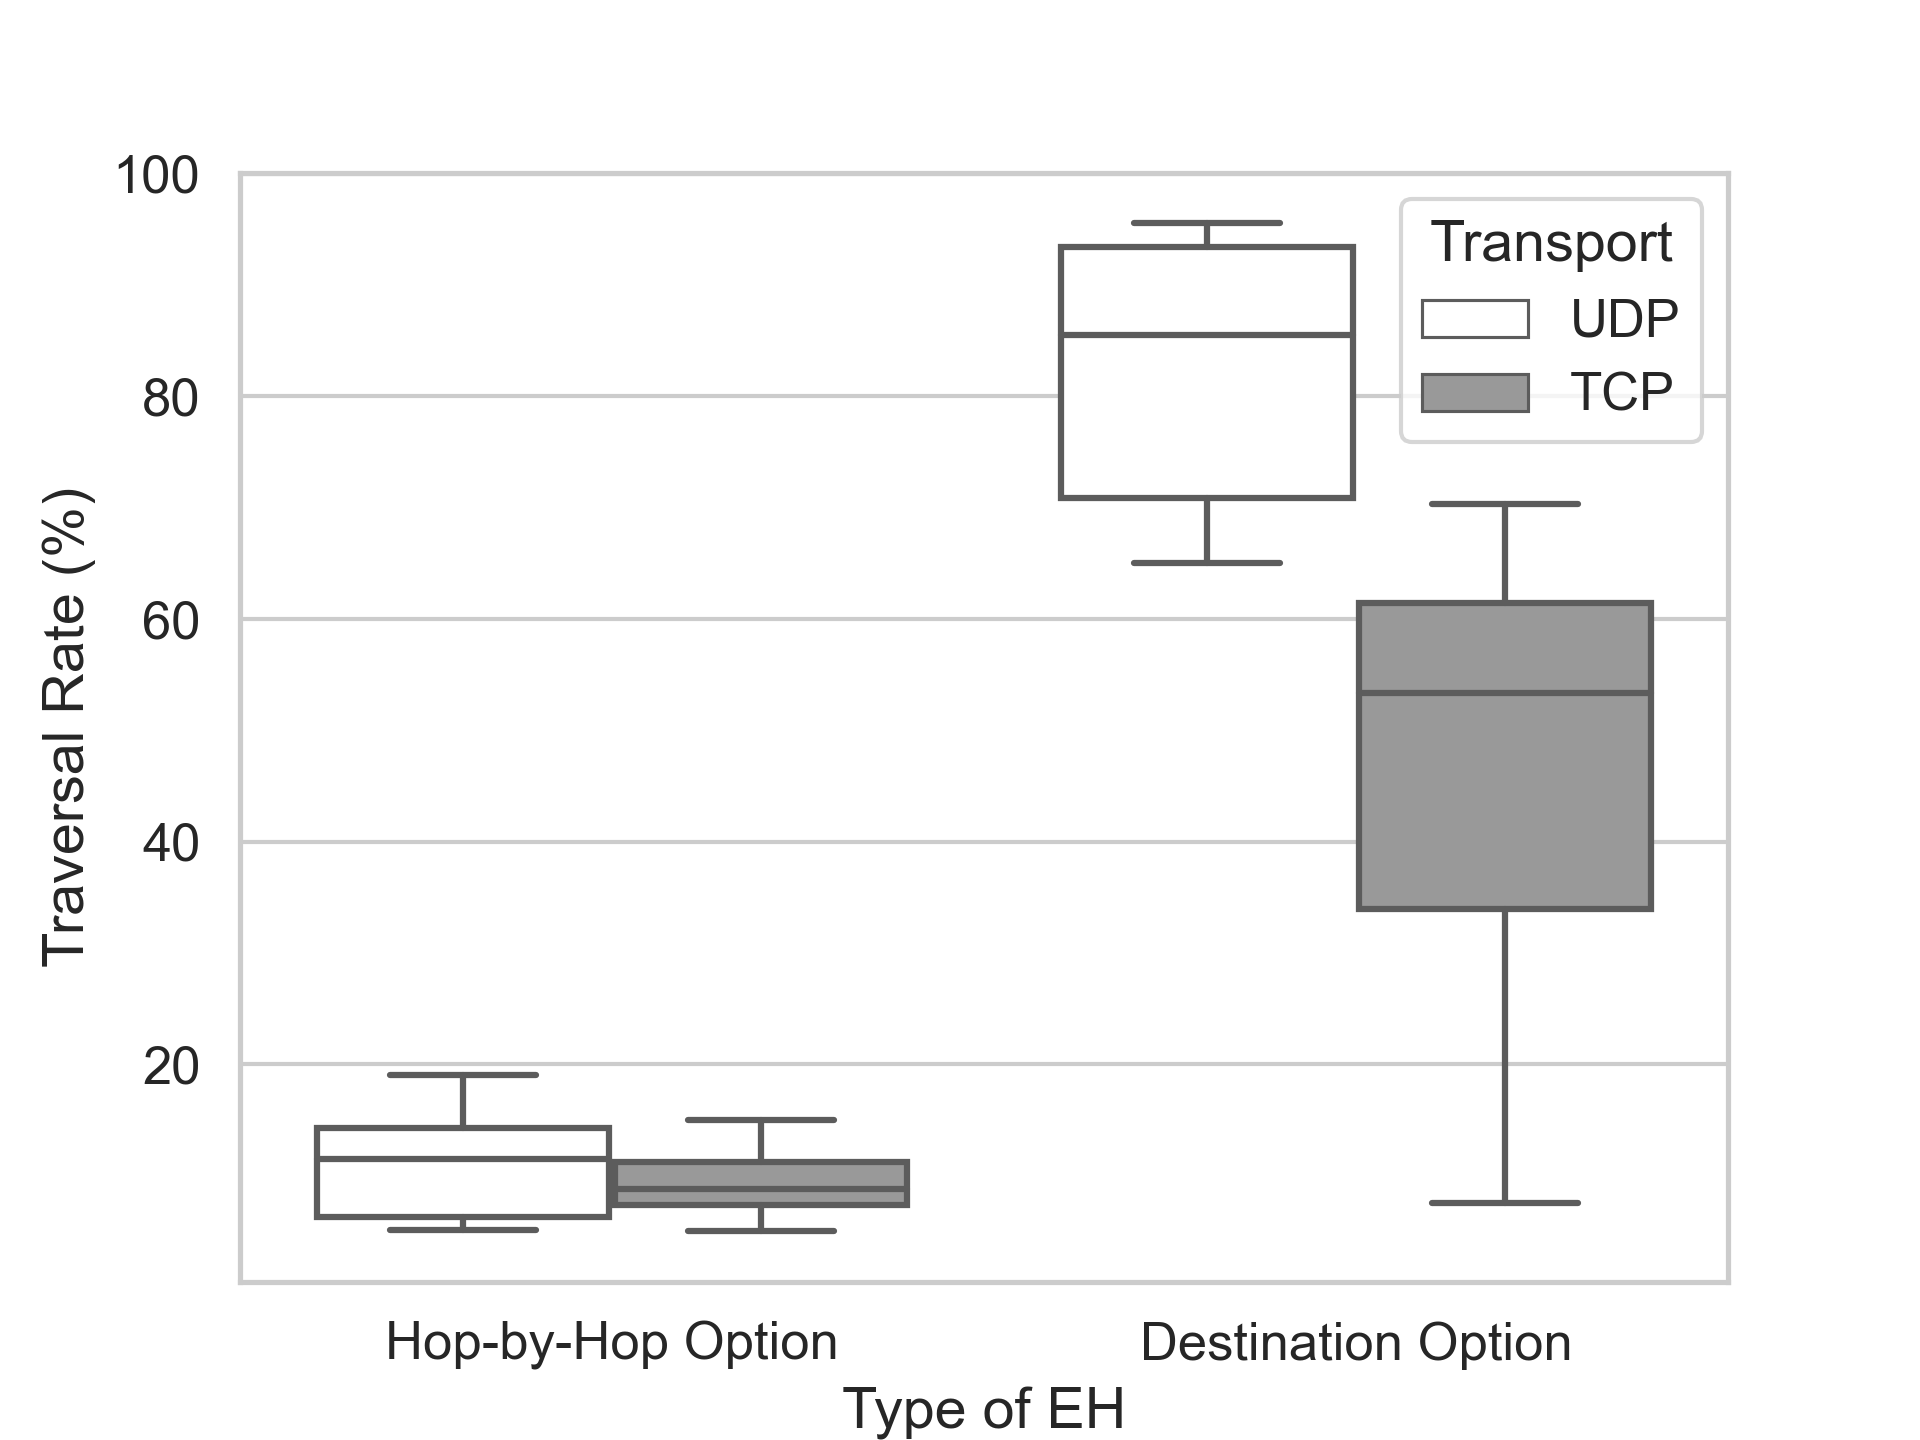
\includegraphics[width=0.5\textwidth]{all_traversal.png}
  \caption{Traversal fro packets including HBH and DST, from Atlas vantage points to target servers located in 7 different countries (dataset R1).}
  \label{fig:countrybox}
\end{figure}

\begin{figure}
\centering
  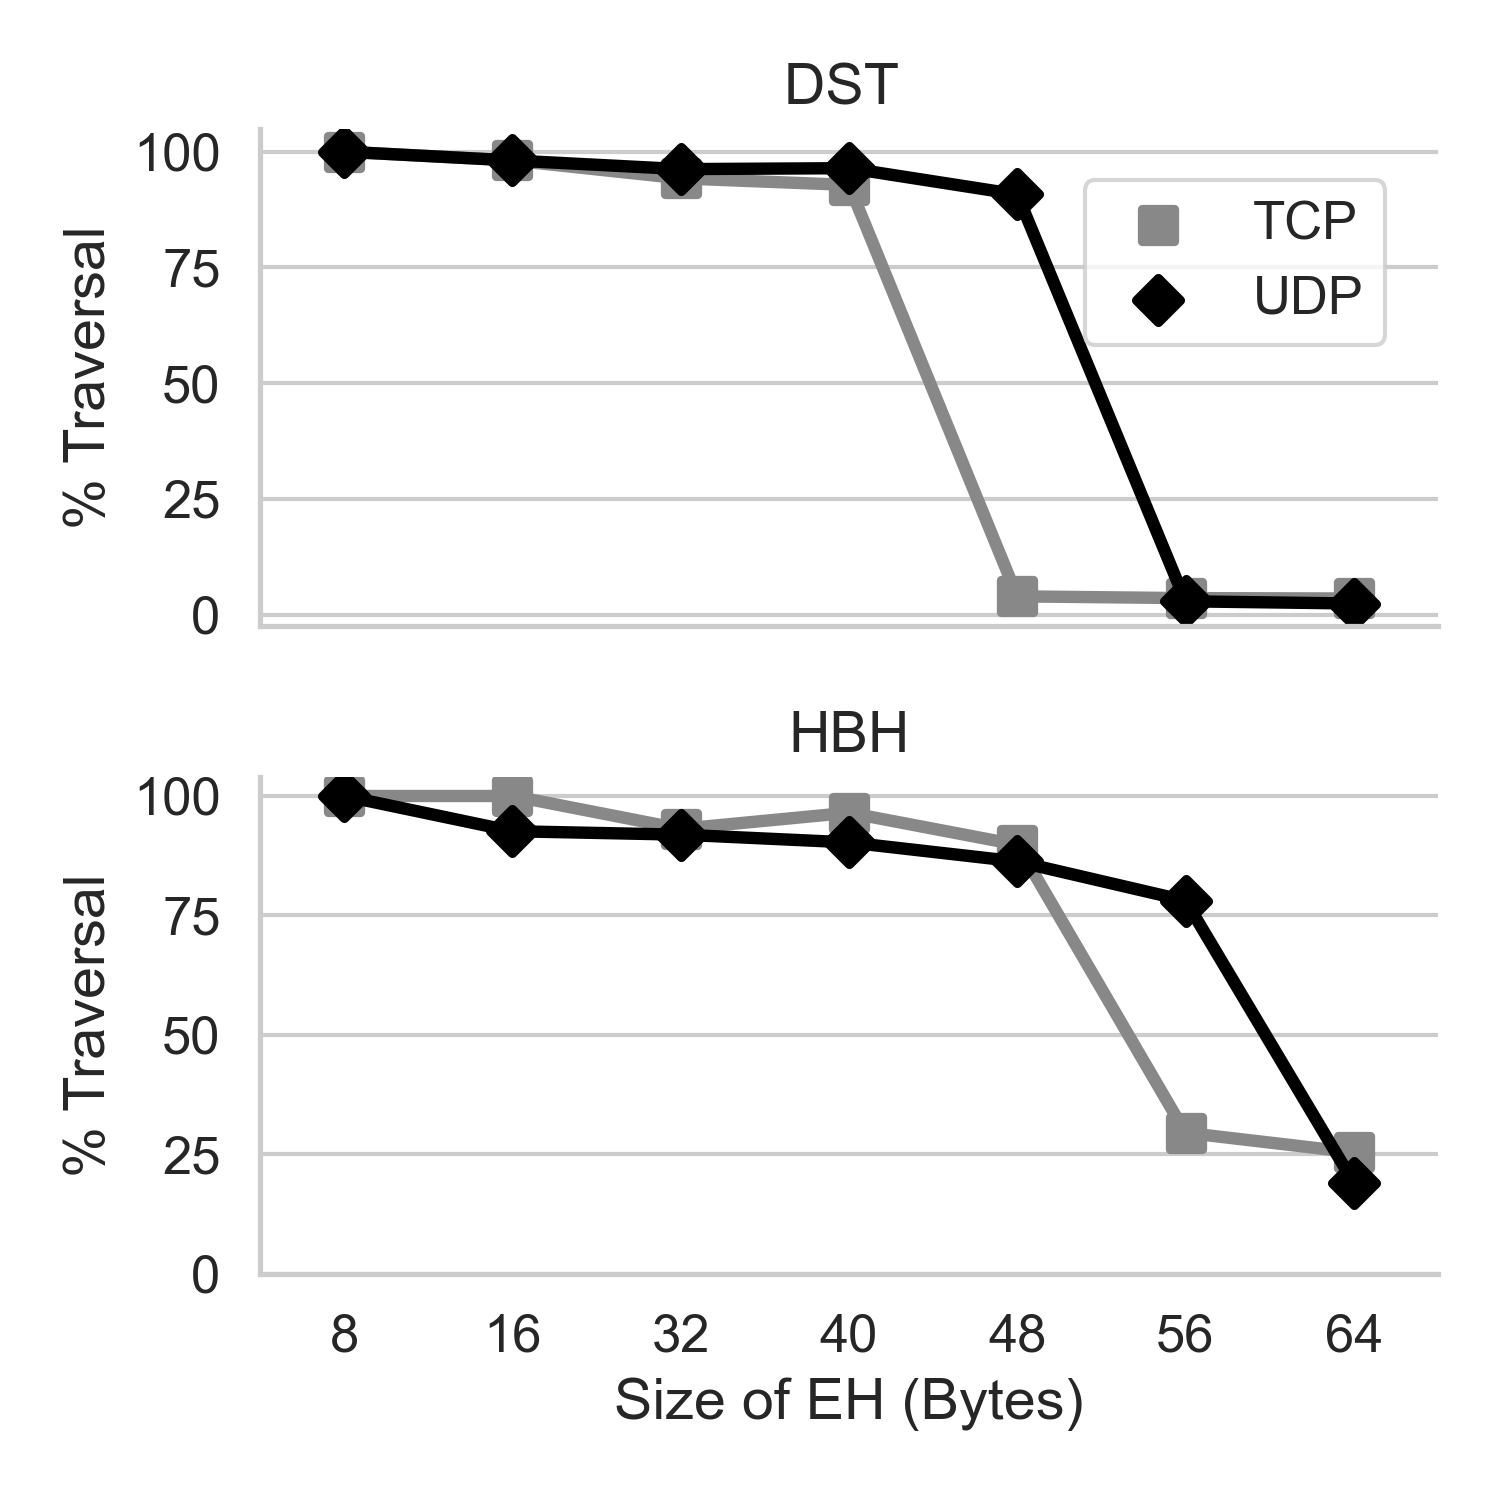
\includegraphics[width=0.45\textwidth]{sizes.png}
  \caption{Traversal for packets including HBH and DST EHs from Atlas vantage points to a target server within the UK JANET network (AS876), shown by size of EH and split by transport.  Total n=129,585 measurements, with a mean of 4628 measurements ($\sigma$=351) for each combination of transport, size and EH  (dataset R2). This variation in the number of measurements results from availability and connectivity of  probes with time.}
  \label{fig:sizes}
\end{figure}

\subsection{Pathologies}
    \label{subsec: pathologies}

The results show low traversal of packets including an EH when using TCP towards the Kazakhstan and Zambian target networks. Both have only one BGP peer, and for both, we find that the majority (over 50\%) of TCP packets see their last reply from a router in the second to last AS on the path (or the destination's upstream AS). In both cases, the traversal to the destination's upstream AS reveals similar results to targets in other tested countries, shown in Figure~\ref{fig:traversal_pathologies}.

\begin{figure}
\centering
  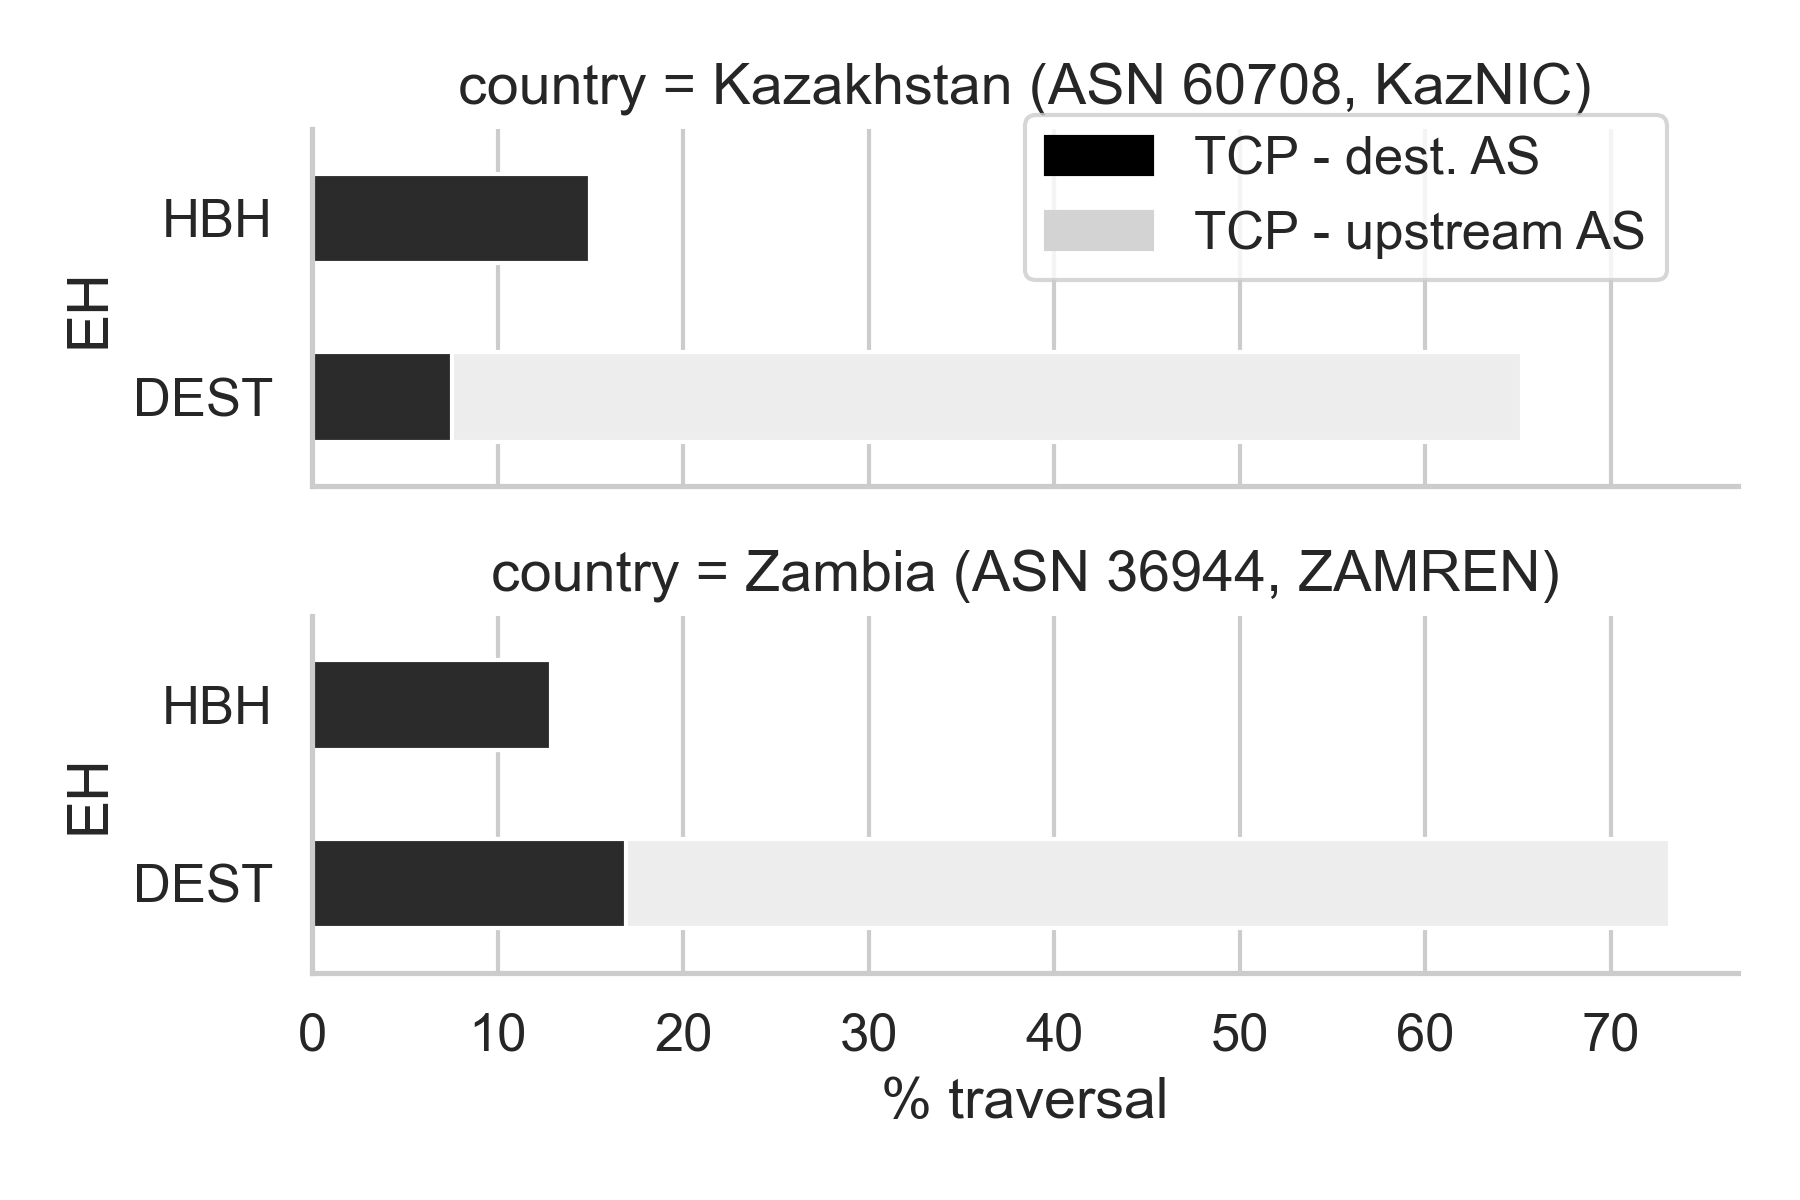
\includegraphics[width=0.5\textwidth]{traversal-pathologies.png}
  \caption{Traversal from Atlas vantage points to both destination and upstream AS for targets in Kazakhstan (n=5075) and Zambia (n=4462). The figure shows the traversal percentage of TCP packets using both types of tested EH.}
  \label{fig:traversal_pathologies}
\end{figure}

Operator mis-configuration can influence traversal: The only BGP peer for the Kazakhstan network is Hurricane Electric (AS6939) and uses a  brokering service where the IPv6 peering is tunneled over an existing IPv4 connection to an endpoint located in Dusseldorf. Upon closer inspection, we find that the 7\% of paths where packets including DST traverse to the destination network originate (with 3 exceptions) in ASes located Australia/New Zealand. The 50\% dropped packets that originate in other geographical areas are filtered at the tunnel endpoint. We therefore assume mis-configuration or a policy within the HE transit network routers results in this pathology. 
%They can also come from comcast but somehow they bypass HE?!?!?!?!


The only BGP peer of the target network in Zambia is Ubuntunet Alliance For Research and Education Networking (AS36944). Over 50\% of TCP packets that include DST are dropped at the last hop seen in this AS. There is no common origin for the results where packets do traverse, suggesting the DST drops are a result of an operator policy. 

\subsection{Path traversal analysis}

Tables~\ref{tbl:uk_as1} and \ref{tbl:uk_as2} present the percentage traversal at each AS on the path to the UK destination for packets including an 8~B EH. We observe the majority of drops occur within the first AS on the path (the vantage point AS) - between 68\% HBH (UDP) and 74\% (TCP) packets and 5\% (UDP) to 25\% (TCP) of DST packets. A difference due to the transport is still observed when the results are split per AS. 

Packet drops within the source AS are common to all Atlas measurements, regardless of destination. Packets including DST and using UDP experience a drop rate less than 1\%, as they traverse further  ASes, suggesting that these packets do traverse the Internet core.

We further investigate cases where packets that include an EH are discarded within the source AS, and find the majority of such drops occur at the first router on the path (i.e. the vantage point's local upstream router).
Figure~\ref{fig:empty_paths} shows the percentages of paths where packets are dropped at this first router - i.e. paths where no traceroute responses are received for test packets, but where responses are received for control packets. Packets that include a HBH are dropped for more than 50\% of paths. The choice of transport has little impact on the result (54\% for UDP and 56\% for TCP, for an 8~B EH). In contrast, between 2 and 15\% of paths drop packets that include a DST, and this rate does depend on the transport: (2.5\% for UDP and 10\% TCP for an 8~B EH). The percentage increases with size  is regardless of which EH was included.


The local routers for this set of vantage points are a diverse mixture of edge routers connecting enterprise LANs, mobile and broadband networks. These routers can also be configured to perform a variety of functions, including access control, and authentication We note that such functions usually require access to transport header information. 

Routers can be configured to perform specific processing on the upper layer (transport) protocols. For example, to avoid the need for Path MTU discovery, it is not uncommon for access network routers to ``clamp" the value of the MSS Option in the TCP header to support encapsulation~\cite{custura-mtu}. 


We do not have a way to determine whether a drop is a result of a configured policy, a bug, or a lack of support. 
However, it is possible to identify paths that insert/modify a TCP option by using a traffic capture tool to examine the measurement packets as they arrive at the destination server during the baseline measurement. By default, the packets sent from an Atlas probe does not include a TCP MSS option - when Option is present at the destination, this means a node on that path has inserted this. We found 853 paths where an on-path router has inserted a TCP MSS option in our baseline measurements to the UK destination. 

We then look at EH traversal within this subset of paths, to determine whether this results in a difference to the overall traversal, on the basis that at least one on-path router will have needed to parse the entire IPv6 Header, including any EHs, to perform this function.
For this subset of paths, we find the traversal is only 2.6\% for HBH and 48.1\% for DST, indicating dropping is more prevalent where an on-path router traverse the EH chain to modify the TCP MSS Option.


\begin{figure}
\centering
  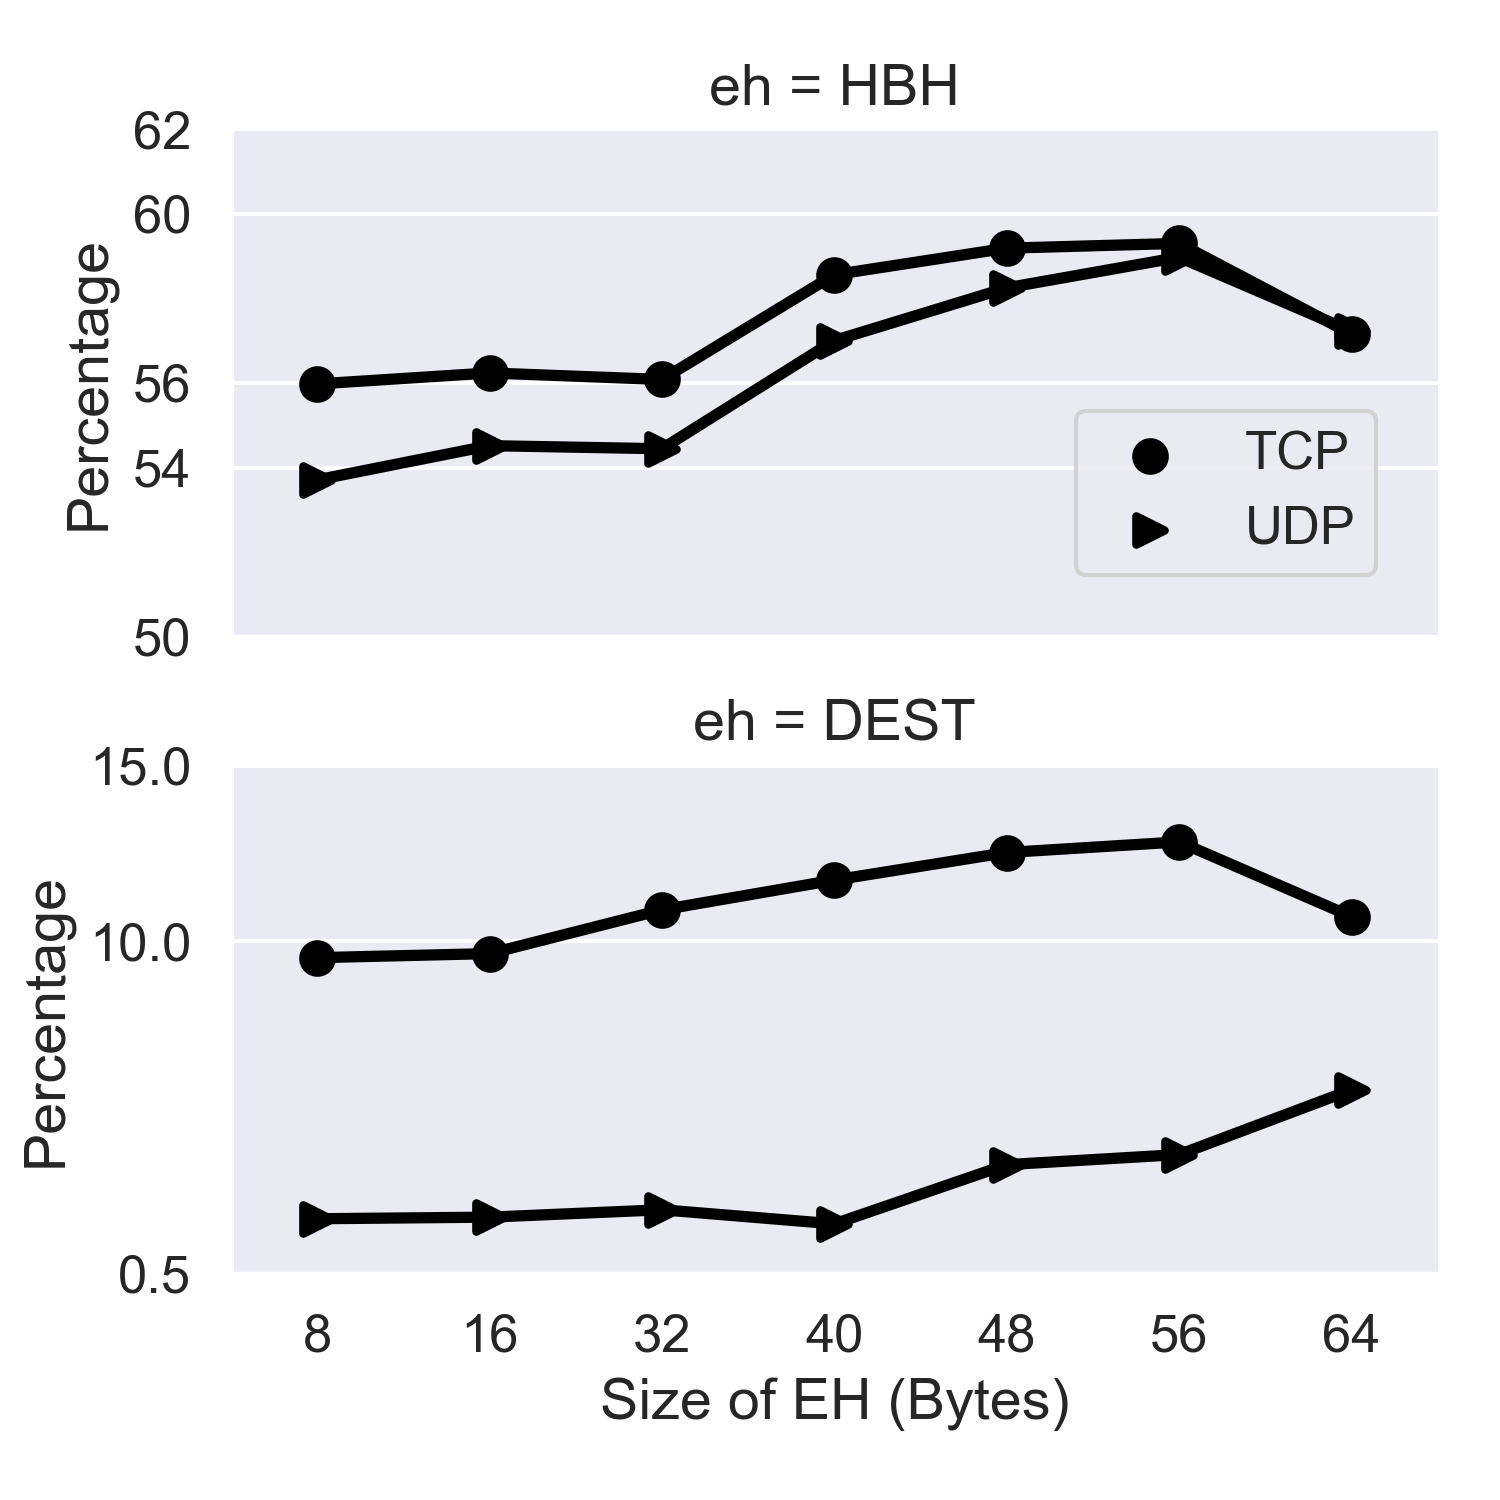
\includegraphics[width=0.5\textwidth]{empty_paths.png}
  \caption{Percentage of paths where packets are dropped at the first router, per EH, transport protocol and size.}
  \label{fig:empty_paths}
\end{figure}


\begin{table}
\centering
\caption{Per-AS drop attribution for 8~B DST packets sent from n=4970 Atlas vantage points to a target destination in AS786. The local AS is responsible for the majority (5\% for UDP and 25\% for TCP) of the drops.}
 \label{tbl:uk_as1}

\begin{tabular}{l|l|l|l}
                                   & 1st AS & AS1\textgreater AS2 & $inf $     \\ \hline 

{Dest UDP 8~B} & 95.3\% & 93\%                 & 91.5\% \\ \hline

{Dest TCP 8~B} & 74.7\% & 70\%                 & 68.5\%
\end{tabular}
\bigskip
\caption{Per-AS drop attribution for 8~B HBH packets sent from n=4970 Atlas vantage points to a target destination in AS786. The local AS is responsible for the majority (68\% for UDP and 74\% for TCP) of the drops.}
\begin{tabular}{p{0.07\textwidth}|l|l|l|l|l}

              & 1st AS & AS1\textgreater{}AS2 & 2nd AS & AS2\textgreater{}AS3 & $inf$     \\ \hline
HBH UDP 8~B & 31.4\% & 20.1\%               & 15\%   & 12.2\%               & 11.4\% \\ \hline
HBH TCP 8~B & 26.9\% & 16.3\%               & 13.9\% & 9.7\%                & 8.6\%  \\ 
\end{tabular}
 \label{tbl:uk_as2}
\end{table}


\subsection{Analysis of chosen path}

Load balancing routers can be configured to read the upper layer headers of a packet. Additionally, many ECMP routers distribute traffic on different paths based on a 5-tuple which includes the Next Header field within the IP header. These routers would send packets without EHs and packets including EHs which are part of the same flow on different paths, and may reduce performance due to reordering.

Some routers can be configured to choose paths based on the Flow Label field in the IPv6 header~\cite{lb-classification}. In this case, adding an EH to a packet within a flow would not result in reordering.

We perform Paris Traceroute measurements to determine whether the choice of path is impacted when a packet includes an EH. This detects the presence of load balancing on a given path~\cite{augustin2006avoiding}, by performing multiple traceroute measurements varying several header fields (a `Paris variation'). A router could be designed to use various fields for load-balancing~\cite{lb-classification}. To identify the packets sent from a specific test, Paris Traceroute identifies each variation based on either the TCP sequence number field or the UDP checksum field~\cite{augustin2006avoiding}.

Six sets of measurements were run from all vantage points to the Zambian destination, with each set of measurement using 16 Paris variations. We select the vantage points and destination based on previous measurements, so as to only measure complete paths, where traversal always succeeds, 766 paths in total. The version of Paris Traceroute that was used to deterministically set the IPv6 Flow Label and transport port number for measurement in a group of set of 16 Paris measurements. The same 16 combinations of IPv6 Flow Label and port number are used for subsequent measurement sets.

\begin{figure}
\centering
  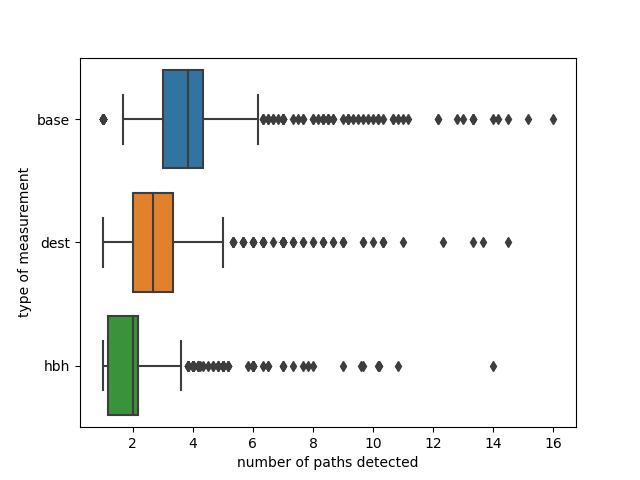
\includegraphics[width=0.5\textwidth]{boxplot-paths-detected.png}
  \caption{Number of paths detected by Paris Traceroute in 866 source-destination pairs, averaged over 5 measurement runs, with each run using the same 16 Paris variations. The baseline measurement using packets with no EH is compared against packets including DST and HBH measurements (dataset R3).}
  \label{fig:paths-detected}
\end{figure}

Figure~\ref{fig:paths-detected} compares how many paths are discovered using Paris Traceroute when using IPv6 packets compared to packets that also include an 8~B DST or HBH EH.
A total of 16 Paris variations discovered on average 4 paths~\cite{augustin2006avoiding}. We reproduce this in our baseline results, finding a median of 4.1 paths. However, the medians for measurements where packets included an 8~B DST or HBH EH are 2.96 and 2.1 respectively (Figure~\ref{fig:paths-detected}).
The difference in the number of detected paths suggests that adding an EH changes the forwarding behaviour of routers on the paths tested.
For 518 (60\%) of source-destination pairs, the measurements sent a packet including a DST EH to detect the same (+-1 path) number of paths as the baseline. For 328 (38\%) pairs, the measurements detect fewer (by 1 path or more) number of paths than the baseline. 
Measurements including HBH EHs detect the same (+-1 path) number of paths as the baseline for only 115 (13.4\%) source-destination pairs. More commonly, fewer paths are detected compared to the baseline when this type of EH is included. This happens on 604 paths (69.7\%). This pathology could happen, for example, if ECMP-enabled routers use bytes from a fixed position in the packet (byte offset) expected to contain the transport ports for their hash calculations, instead of parsing the IPv6 header chain. 

This means that packets including a HBH EH are less likely to take the same Internet path as packets with no EH, and less likely to take advantage of path optimisations.

For some source-destination pairs, the EH Paris measurements detect at least 1 more path than for a packet with no EH.  These cases are rare - around 1\% (8 paths for DST and 10 for HBH), but can reveal interesting pathologies.
For example, for one pair the baseline measurement detects 4 paths, the DST measurement detects 2 paths, while the HBH measurement detects 14(!) different paths. Upon closer inspection we find a single router that enumerates 14 interfaces, only in the presence of packets containing HBH EHs. While this does not likely impact usage (the paths converge again at the next hop), it is not expected behaviour.


For 10 source-destination pairs in our dataset, some of the paths discovered for each pair drop packets including an HBH EH - and so packets including this EH can not expect to consistently travel between the source and the destination. 
%For 12 source-destination pairs in the dataset, not enough data was gathered using Destination Option EHs to complete a measurement run. Not enough data was gathered for 137 (15.8\%) pairs.

This set of measurements indicates that packets including HBH and DST EH are forwarded the same way as packets without EHs on only 13\% (in the case of HBH) and 60\% (in the case DST) of paths respectively, and that adding an EH can impact the function of load-balancing routers.
 
\section{Pathspider results} 
\label{sec:pathspider-results}

This section presents the results obtained from the
PATHspider~\cite{learmonth2016pathspider} dataset. The objective of these
experiments is to observe the responses of DNS servers when probed with a DNS
query, both with and without EHs. In essence, these tests concentrate on
analyzing the behavior of endpoints rather than the behavior of routers along
the path. The PathSpider dataset, in comparison to the Atlas dataset, employs a
smaller number of vantage points but encompasses a larger number of target DNS
servers. The list of DNS servers includes all the authoritative Name Servers (NS) of the Cisco
Umbrella top 1M domains.

For each identified authoritative NS, PathSpider first performs a control
measurement by sending a DNS query without EH.  This step ensures that the DNS
server supports the intended destination. The test is then repeated, including
a PadN DST or a HBH extension. The test is considered successful if the server
responds to the DNS query both with and without EH. For web server
destinations, PathSpider sends a TCP SYN packet and considers the test
successful if the server replies with a SYN/ACK.

%This section reports the end-to-end support percentage, indicating the paths
%where test packets receive a response from the destination server.

\begin{table} 
\centering
\begin{tabular}{c|cc|cc}
\multicolumn{1}{l|}{} & \multicolumn{2}{c|}{DST Traversal} & \multicolumn{2}{c}{HBH Traversal} \\ \cline{2-5} 
\multicolumn{1}{l|}{} & \multicolumn{1}{c|}{TCP}       & UDP      & \multicolumn{1}{c|}{TCP}     & UDP     \\ \hline
UK                    & \multicolumn{1}{c|}{69.1}      & 69.3    & \multicolumn{1}{c|}{12.5}    & 15.8  \\ \hline
Canada                & \multicolumn{1}{c|}{76.3}      & 76     & \multicolumn{1}{c|}{23.3}    & 24.2  \\ \hline
Australia             & \multicolumn{1}{c|}{72.5}        & 72.2      & \multicolumn{1}{c|}{17.7}    & 17.5  \\ \hline
Singapore             & \multicolumn{1}{c|}{72.8}      & 72.7    & \multicolumn{1}{c|}{17.4}    & 17.4   \\ \hline
Poland                & \multicolumn{1}{c|}{76.5}      & 76.8   & \multicolumn{1}{c|}{24.4}    & 24.7   
\end{tabular}
\label{tbl:e2e_traversal}
\caption{End-to-end traversal for an 8~B Pad N Option for packets including Dest and HBH EHs, from vantage points in 5 countries to n=18002 unique authoritative NSes in the Cisco Umbrella Top 1M, in 2787 different known ASes. All measurements were performed in February 2023, part of dataset P1. }
\end{table}

\begin{table} 
\centering
\begin{tabular}{c|c|c|c}
           & \% of dataset &  DST Traversal & HBH Traversal\\
\hline
Cloudflare & 18                      & Yes                & No                 \\
\hline
Amazon     & 11                     & No                 & No                 \\
\hline
Hetzner    & 3                     & Yes                & No                 \\
\hline
Gandi      & 4                     & No                 & No                 \\
\hline
Ionos      & 3                    & Yes                & No                
\end{tabular}
\label{tbl:provider_support}
\caption{End-server support for DST and HBH for major DNS server providers, n=99,987 paths, based on measurements from December 2022. 
%Google does not support either EH, and is not listed in the table because it was only 30 destinations in the dataset.
}
\end{table}

\subsection{End-to-end support}
\label{subsec:e2esupport}

Table~\ref{tbl:e2e_traversal} show the percentages of successful test with the
DST and HBH EHs for both TCP and UDP DNS queries across the whole set of
authoritative NS for the current Cisco Umbrella top 1M Domains list (updated at
February 2023).
% ANA TODO - double check results^

Similar to results previously presented for access networks, server support
varies between the DST and HBH EHs: 69 to 80\% of the tested servers replied to
packets when including DST, and up to 24.2\% do so when including HBH. The
traversal does not vary with the transport (as seen for the access network
results in the previous section). We attribute this to the lack of the type of
local routers (i.e. CPEs) normally present in access networks. 

Only one measurement, from the Singapore vantage point, observed a 5\% difference based on transport in favour of TCP for both tested EHs.
Finally, the table shows variations in support based on vantage point - support varies between 12 to 24.7\% for HBH, indicating fewer packets were dropped in transit networks in the latter case.

However, around one third of destinations in the DNS dataset featured in Table~\ref{tbl:e2e_traversal} are hosted by a few major hosting companies (Cloudflare, Amazon, Gandi etc.), which employ network policies that filter packets that include EHs. 

End-server support for major DNS server providers are presented in Table~\ref{tbl:provider_support}. In Early December 2022, Cloudflare servers started responding to DNS queries sent with packets including DST, this results in a jump from 57\% to over 70\% for the dataset. If all major providers would enable support, this would bring the success of the E2E test to over 90\% for DST and 60\% for HBH for this dataset.

We tested end-to-end support for webservers in the Cisco Umbrella top 1M Domains list (232,350 unique IP addresses, Feb 2023) from the same destinations. This list of webservers is dominated by a few major hosting companies: around 52\% of destinations are hosted by Amazon Inc (AS16509); 23\% are hosted by Cloudflare (AS13335), and around 2.5\% each are hosted by Akamai Technologies and Google. We break down the supported EHs for each in Table~\ref{tbl:web_provider_support}. We find more than two-thrids of Amazon-hosted webservers respond to connections by packets including DST, in contrast to Amazon-hosted DNS servers, where none do. 

Overall, we find end-to-end support for all tested webserver addresses to be between 72 and 78\% for  packets including DST and between 2-3\% for HBH.


\begin{table} 
\begin{tabular}{c|c|c|c}
           & \% of dataset & DST Traversal & HBH Traversal\\
\hline
Amazon & 52                      & Yes                & No                 \\
\hline
Cloudflare     & 23                     & Yes                 & No                 \\
\hline
Akamai    & 2.7                     & Yes                & No                 \\
\hline
Google      & 2.3                     & No                 & No                 \\
\
\end{tabular}
\label{tbl:web_provider_support}
\caption{End-server support for the DST and HBH for major webserver providers, n=99,987 paths, based on measurements from December 2022. Google does not currently support either EH, and is not listed in the table because it only had 30 destinations in this dataset.
}
\end{table}


\subsubsection{Option Type support}

The next set of tests evaluate support for different Options. We repeated the DNS server experiment described above from one vantage point, but also varied the Option Type and Option Length fields. 
Table~\ref{tbl:option_type_support} shows the support for different Option Types within the authoritative NSes for the current Cisco Top 1 Million Domains. We test a well-known Option, PadN~\cite{rfc2460}, against a recently-standardized one - MinPath MTU HBH~\cite{rfc9268}. We also test two experimental Options, 30 and 254~\cite{RFC4727}. The latter was chosen to test the traversal when the Option Type has its two most significant bits set.
We find that the type of Option  does not affect traversal where the two most significant bits of the field are not set - with the same traversal percentage for PadN, minPMTU and the Experimental Option 30. Where the highest order bits are set, traversal is expected to be 0~\cite{RFC8200} - however, we  receive responses for 0.4\% of paths, indicating all routers on that path have ignored these bits.

We tested an incorrectly set Option Length field. Any node parsing this EH field should validate the Option Length set for each Option, traversal is expected to be 0~\cite{RFC8200}; however we also find a small number of paths (0.5\%, or around 80 paths) where all routers on the path ignore this field.

\begin{table}
\begin{tabular}{l|l|l}
Test                      & DST Traversal & HBH Traversal\\
\hline
Pad N Option (1)          & 69.3           & 15.1          \\
PMTU Discovery (48)       & 69.5           & 15.8          \\
Experimental Option (254) & 0.4            & 0             \\
Experimental Option (30)  & 69.4           & 15.1          \\
Incorrect Option Length   & 0.5            & 0.05            
\end{tabular}
\label{tbl:option_type_support}
\caption{End-to-end support for different Option Types in the authoritative NSes for the Cisco Top 1 Million Domains, n=19052 unique IPv6 targets using a UDP transport (dataset P2).}
\end{table}

\subsubsection{ICMP Unreachable Messages}

We also tested the generation of
ICMP messages, by observing if an ICMP message is returned when a packet including a HBH is dropped by the path. ICMP unreachable messages are seen on 0.2\% of the tested NS paths. For packets including DST, ICMP unreachable messages are seen on 0.3 – 8.8\% of paths, depending on the vantage point.
This suggests that ICMP messages cannot be used to ascertain whether a packet was dropped in transit due to the presence of Options.
Upon closer inspection, we also find that for all destinations, ICMP unreachable messages can be received even when the test succeeds on up to 2\% of paths. These are exclusively received from routers in destination ASes and are a result of incorrect processing~\cite{RFC8200}.

\subsubsection{ICMP Parameter Problem Messages}

When a packet includes a Dest or HBH that sets the two MSBs, a router that does not understand this Option should discard the packet and return an ICMP Type 4 Parameter Problem message to the sender~\cite{RFC8200}. To examine whether this is prevalent in the Internet, we repeat the DNS server experiments using packets that include experimental Option Type 254. This Option has its two MSBs set and is unlikely to be understood by any router, and therefore we expect all sent packets to be dropped.

Results for DST and HBH are described in Table~\ref{tbl:icmp_support_dst}.
In the case of DST, for all vantage points tested, only the local router at the vantage point returns ICMP Type 4 Parameter Problem messages for the packet, as expected; the percentage of destinations for which the ICMP messages are received varies between 50-100\%. Because the local router always generates these messages, this variation may be due to ICMP rate-limiting. 
The local router forwards packets that include HBH,  ICMP Type 4 Parameter Problem messages that are received from routers on the path or in the destination AS. The response rate is 52 - 73\%. 

For both tested EHs, ICMP rate-limiting and filtering is evident. Therefore, ICMP is not a reliable indicator of whether a packet was dropped with an unknown Option that sets its two MSBs. We also find many of these paths continue to forward packets packets regardless of the setting for the 2 MSBs.

In addition, between 0.2 and 0.5\% of paths for packets including DST, we also find that despite sending this ICMP message, the local router also forwards the packet to the destination and a response is  obtained from the server (the end-to-end test succeeds). This indicates some routers do not process packets as specified by~\cite{RFC8200}.

\begin{table}
\begin{tabular}{p{0.12\textwidth}|p{0.04\textwidth}|p{0.03\textwidth}|p{0.03\textwidth}|p{0.03\textwidth}|p{0.03\textwidth}|p{0.025\textwidth}}

\centering

                                           &             & UK        & Can       & Aus    & Sgp          & Pol     \\
                                           \hline

{\% ICMP received from vantage AS}        & {HBH DEST} & {0 100}  & {0 51.6}    & {0 51.9}    & {0 51.9}    & {0 51.5}  \\
\hline
{\% ICMP received from elsewhere on path}          & {HBH DEST} & {72.8 0} & {52.5 0}    & {68.2 0}    & {69.2 0}    & {73  0}    \\
\hline

{\% ICMP received, packet forwarded}          & {HBH DEST} & {0 0.52} & {0 0.48}    & {0 0.46}    & {0 0.24}    & {0 0.46}  \\
\hline

{\% ICMP message not received} & {HBH DEST} & {27.2 0} & {47.5 48.4} & {31.8 48.1} & {30.8 48.1} & {27 48.5} 
\end{tabular}
\caption{The set of behaviours for ICMP processing.}
\label{tbl:icmp_support_dst}
\end{table}


\subsubsection{Longitudinal analysis of support for EH}

Table~\ref{tbl:longitudinal_support} presents a longitudinal set of measurements across the same set of domains collected over 3 years. Each domain was resolved prior to the measurement, resulting in a variation of the total unique IP addresses tested, presented in the last table row. The results show a decreasing trend in  support for HBH, with DST support remaining constant over time, until December 2022 when Cloudflare enabled support, as described in Subsection~\ref{subsec:e2esupport}.

% Ana: verify total number of paths.
\begin{table}
\begin{tabular}{l|l|l|l|l}
                    & Jan 2020 & Jul 2020 & July 2022 & Dec 2022 \\
\hline
DST Traversal& 59.9\%   & 54.3\%   & 57.4\%    & 71.7\%   \\
HBH Traversal & 25.7\%   & 23.8\%   & 16.4\%    & 11.9\%   \\
\hline
Unique IP addresses & 18296    & 19690    & 19553     & 20050   
\end{tabular}
\label{tbl:longitudinal_support}
\caption{End-to-end support for an 8~B Pad N Option for both Dest and HBH EHs, from one vantage point to the authoritative NSes for the same set of 1M domains, between Jan 2020 and Dec 2022 (dataset P1). The transport used was UDP.}
\end{table}

\subsection{AS analysis}

Table~\ref{tbl:as_pathspider} presents ASes targeted by Pathspider (2868 in total) alongside evidence that they support either the DST or HBH EH.
If at least one reply is seen from an AS to one of our test packets from any of the locations tested, we consider that AS supports the traversal of packets that include the tested EH type. Thus, at least 92.4\% of destination ASes allow traversal of packets including an 8~B DST EH, and more than half, 53.8\%, allow an 8~B HBH EH. This  reduces when the packet travles though multiple ASes towards the destination, revealing that many packets that include an EH are dropped in an AS that is different from the destination AS. For DST, 3.4\% fewer ASes permit DST traversal on more than half the paths, whereas for HBH, the difference is 16.6\%.
When only considering the subset of ASes (1606) tested over 10 or more paths, the results vary little: at least 93.2\% of destination ASes allow traversal of packets including an 8~B DST EH, and more than half, 55.9\%, allow an 8~B HBH EH.

    \begin{table}
\begin{tabular}{p{0.195\textwidth}|p{0.11\textwidth}p{0.118\textwidth}}
                                          & Paths per AS$>$=1 & Paths per AS$>$=10 \\ \cline{1-3} 
Total number of ASes                      & 2787                                            & 1606                                            \\ \hline
AS does not support DST               & 212 (7.6\%)                                     & 110 (6.8\%)                                     \\
AS supports DST on 1 or more paths   & 2575 (92.4\%)                                   & 1496 (93.2\%)                                   \\
AS supports DST on 50\% paths or more & 2476  (88.8\%)                                  & 1437 (89.4\%)                                   \\ \hline
AS does not support HBH               & 1287 (46.2\%)                                   & 709 (44.1\%)                                    \\
AS supports HBH on more than 1 path   & 1500 (53.8\%)                                   & 897 (55.9\%)                                    \\
AS supports HBH on 50\% paths or more & 1037 (37.2\%)                                   & 580 (36.1\%)                                   
\end{tabular}
\label{tbl:as_pathspider}
\caption{Number of ASes where DNS servers can be reached via packets including either Dest or HBH. The first column considers all destination ASes in the dataset, while the second only looks at ASes that host 10 destination addresses or more. Based on measurements from December 2022 (dataset P1).}
\end{table}

\section{Discussion} 
\label{sec:discussion}

Since its standardisation, the IPv6 protocol has
seen widespread adoption~\cite{v6adoption_ton} and the hardware and software that
support it have also matured: packet parsing capabilities in routers are increasing and
router architectures have evolved~\cite{metamorphosis, hauser2023}, including some solutions based on hardware and re-configurable
logic that can enable new functions to be introduced~\cite{cisco-silicon-one}. Updates also have been made to the IPv6 standard based on operational experience~\cite{RFC5722}~\cite{RFC6946}~\cite{RFC6564}~\cite{RFC8200}.
The following sections discuss the usability EHs on Internet paths and the barriers to introducing new Options.

\subsection{Usability of EH across Internet Paths}

EH processing has become a recent focus in the standards community~\cite {ietf-v6ops-hbh-03}, where new applications are emerging. Many of the current deployment scenarios are within a single domain. There are proposals to help facilitate an increase in support for EH~\cite{ietf-6man-HBH-processing-06, ietf-6man-eh-limits-02}. 
So, it is timely to ask what is the prospect for using EHs to extend IPv6 across adjacent domains across end-to-end Internet paths?

First, we consider whether EH would traverse an Internet path.
We find that packets that include the DST EH traverse up to 96\% of Internet paths~\ref{fig:countrybox} and that over 92\% of server edge ASes~\ref{tbl:as_pathspider} also support DST.

%Question 1:  Is there a longitudinal trend making this more easy or harder?
We also find that packets that include HBH EH are still currently dropped in many transit networks (validated in Table~\ref{tbl:as_pathspider}) and in access networks in Figure~\ref{fig:countrybox}. Mis-configuration or other network policies also result in various pathologies within transit networks, shown in Subsection~\ref{subsec: pathologies}. 

We also find that traversal reduces significantly for packets that include EHs (both DST and HBH) when a path contains edge-network routers that insert a TCP transport option.

Server-side, testing for the same set of NSes between 2019 and 2022 reveals the support for 8~B PadN HBH decreases over time when considering individual destinations (Table~\ref{tbl:longitudinal_support}), as more NS servers become centralised under only a few ASes that do not support HBH.  However, an analysis of AS results reveals more than half of the tested ASes allow packets that include a HBH EH, and confirms that transit networks can present an obstacle to deployment of the HBH EH.

RFC 7872~\cite{RFC7872} describes the traversal to the authoritative NSes for the Alexa Top 1M domains in 2014. This observes packets including an 8~B PadN DST traverse paths to 78.6\% of NS destinations and packets including an 8~B PadN HBH traverse paths to 45.9\% of destinations. These results were measured from a single vantage point and are not grouped per AS, and can only be compared with results in Table~\ref{tbl:longitudinal_support}, which indicates a 5-9\% decrease in support for DST and a 25-30\% decrease in support for HBH, although we note this could reflect the choice of vantage point or changes within the top 1M domain list itself between 2014 and 2023.
As the AS analysis reveals that packets that include an EH traverse to up to 90\% and over 50\% of ASes respectively, we can infer the decrease is due to drops within the destination AS.

%Question 2: is there a limit to extension headers that prevents them from traversing certain Internet paths such as limiting length of the EH chain or a specific EH length? Would ? Is it different between HBH and DO?

XXX Do we have a short statement on use between a set of adjacent transit domains? XXX

To understand if traversal can be improved by limiting the size of the total EH Chain, we explored using different size of EHs and found that EH Chains of up to 40~B   have the highest probability of traversing an access network path with a UDP transport, shown in Figure~\ref{fig:sizes}.

This suggests that when using an EH, keeping the packet size under this limit would help in ensuring consistent deployment.

In some cases, low traversal was attributed policy-based dropping, and using ACLs may be necessary in some networks today to protect routers (e.g. where EH processing leads to DoS vulnerabilities or undesirable side-effects~\cite{passive-threats}). In cases where this is not needed, such a policy is not desirable, because it results in ossification that will obstruct new uses of EHs.

% XXX A way forward is to skip the EH to facilitate HBH support and still protect the control plane

% makes sense to use them within domains, where encryption is not needed, but perhaps in an 'untrusted' domain quic etc is better


%Question 6: what is the opportunity for destination options? Is it a good trade-off to have a network layer? That is consistent transport header or is it wiser to put the transport header information within the transport and therefore allow it to be encrypted such as quic transport parameter - so what is the real advantage of destination options?


%Question 3a: When options extension headers do traverse, do they traverse consistently for the same pair of endpoints?

%Quetsion 3b: Does the flow label help to ensure a consistent set of network routers on a path? -- If not, then we ought to suggest the step towards evolution would be to add a PAD option to all packets that would not otherwise have an EH?
%Question 3c: Is there a trend to set meaningful entropy in the flow label against the original place where many endpoints sent a zero value flow label?
%Question 3d: Is the flow label invariant .... is the FL the same at src as at the dst ...  (i.e. do devcies on-path rewrite) is that something RIPE could easily answer. - If they reset to zero then they are evil!
%Here we should not forget the proposals to add flow metadata as a hop by hop extension to let network routers know helpful information to help forwrad the packets in a flow.

%Question 5: If we find HBH don’t work everywhere then ….What is the opportunity for using a hop by hop extension header on some of the packets belonging to a flow? does this result in new forwarding pathologies? That is where the packets that include EHs take a different set of routers to the packets with no extension headers, and if so do they take a different network or do they simply follow a different path through the same operator network? Does this result in inconsistent loss? Is the option useful ?

Results presented in Figure~\ref{fig:paths-detected} show that including an DST or HBH EH in a packet can change its forwarding path. Our experiments varied both the Flow Label and the source port of packets to detect if this influenced the path between the endpoints. We discovered this variation and attribute this to the position of the EH between the IPv6 header (which contains the flow label) and the transport header (which contains the transport port), suggesting some load-balancing network equipment do not skip the header chain to find the actual port information, but might instead wrongly use a byte offset to the expected position of the source port. Overall, this means traffic flows that use a mix of packets that include an EH and packets without, must take care as these packets may not travel on the same Internet path, resulting in reordering or differences in patterns of loss/delay. 

XX Is there ANYTHING we can cite on Flow Label trends? Is this helpful: https://ieeexplore.ieee.org/document/7014534  XXX

\subsection{Potential to introduce new Options}

We next determine whether new Options could be defined and used across the Internet.

We find that traversal does not depend on the type of Option  (see Table~\ref{tbl:option_type_support}). This is important because it suggests a new DST or HBH Option can be defined and then used on any path that supports EH processing. 
However, since it seems currently unlikely that all routers on a path will support a specific HBH Option, functions that use an Option need to be designed to be robust to routers skipping HBH processing (e.g., the MinPMTU  Option~\cite{rfc9268,rfc9343}. 

XX What was the para below intended to say, it seems to contradict XX

Our results also show that when an Option is encountered that cannot be processed,
most routers are configured to discard packets and to send an ICMP message, as specified by~\cite{RFC4443}. However, we did find instances where the router (correctly) sends an ICMP message in response to a DST EH that has both of the most significant bits set, but nevertheless forwarded the packet; more commonly, packets that include a HBH EH with both most significant bits set are forwarded (without sending an ICMP message). Overall, ICMP is not found to be a reliable mechanism for indicating whether or not packets including an EH is forwarded. This suggests that this part of the specification is not a  reliable method for detecting whether a path can implement a new function.

Instead, we suggest it is possible to incrementally extend IPv6 by only including an EH when a path is found to support them. 
An application can be designed to first send a test packet including an EH with the required Option, or combination of Options, and not send additional packets that include this EH until the test packet is acknowledged. The process of sending packets both with and without a specific header to discover whether a path can support a specific header is sometimes called "racing" (e.g., transport protocol racing is explained in~\cite{ietf-taps-arch-18}. This resembles "A/B protocol feature testing", as used in Pathspider~\cite{learmonth2016pathspider}).

%% ADD here some numbers for racing --what happens on rest of path if the traversal is ok at the first AS
Since the set of routers forming a path can change with time, this discovery process ought to be repeated from time-to-time. 

\section{Conclusion}
\label{sec:conclusion}

Across the Internet, we find traversal of HBH and DST is variable depending on EH, size, transport and type of network. We find these EHs can impact the function of load balancing routers and that of routers which modify transport headers. We conclude that deploying them in the Internet needs to take into account the type of network these will travel over, and carefully consider whether to add them to packets in a stateful flow.


Packets including DST can already traverse many paths both within the core of the Internet, and at the server and network edge. In the case of packets including HBH, 
EH processing has become a recent focus in the standards community, aiming to motivate the implementation of router architectures that facilitate it~\cite{ietf-6man-HBH-processing-06, ietf-v6ops-hbh-03, ietf-6man-eh-limits-02}. 
It is expected this will help foster the development of new Options and motivate a shift to more permissive network operator policies.

In summary, we suggest there is opportunities to use IPv6 beyond a single controlled domain, with the
expectation that applications incrementally utilise new features using HBH and DST EHs, and provide recommendations for the design of  features that need to account for routers that may skip EH or block packets that include EH.

\section*{Acknowledgements}

The authors appreciate the valuable comments provided by Justin Iurman and Benoit Donnet and Eric Vincke. This work has been partially supported by the University of Aberdeen's School of Engineering Department, and partially funded by the RIPE
NCC Community Fund, Project ID 619935.

\bibliographystyle{abbrv}
\small
\bibliography{main,rfc}


\end{document}
